
\appendix

\section{Backup}

\begin{frame}{Experimental data in NNPDF4.0}
    \vspace*{-1em}
    \begin{columns}
        \column{0.48\linewidth}
            {\footnotesize
            \begin{itemize}
                \item 44 new datasets included
                \item 323 more data points in NNPDF4.0 \\ than in NNPDF3.1
                \item New data is mostly from the LHC RUN II
            \end{itemize}
            }
            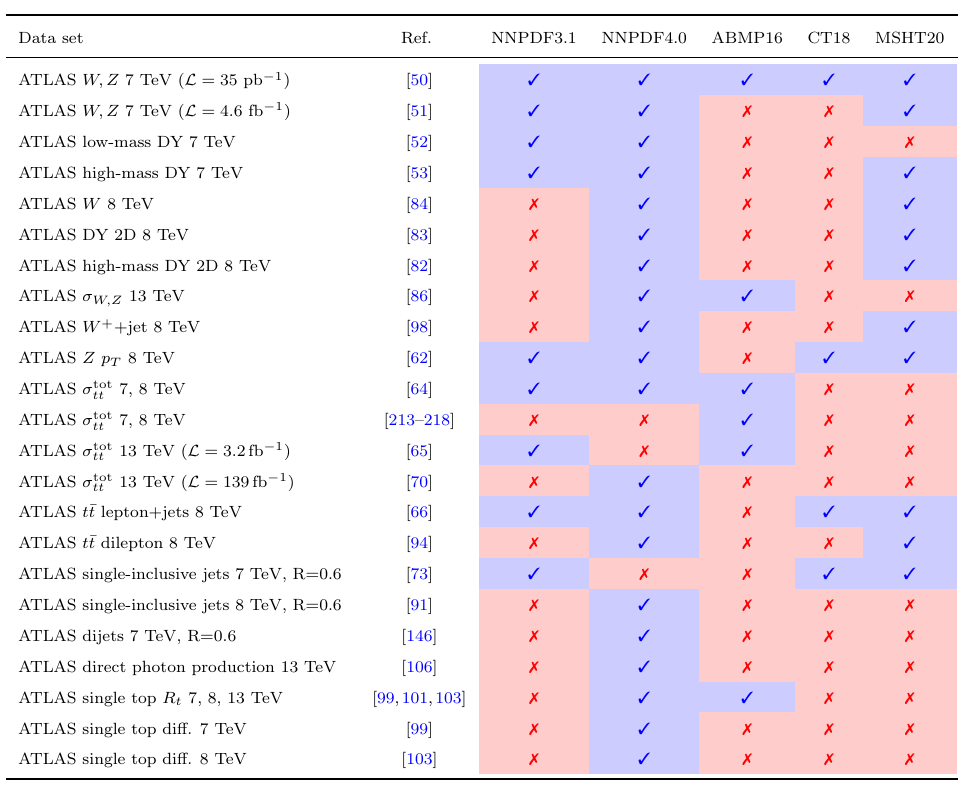
\includegraphics[width=0.9\textwidth]{atlas_data_table}
    
        \column{0.48\linewidth}
            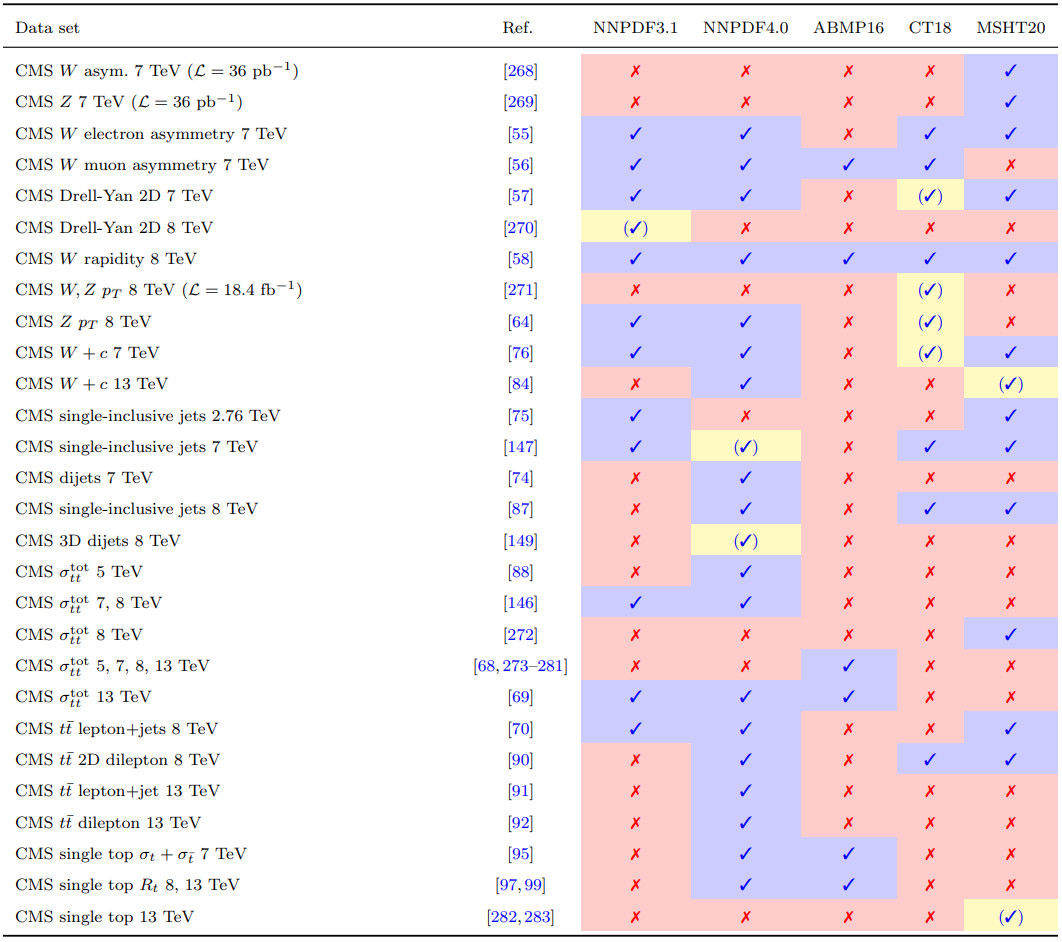
\includegraphics[width=0.9\textwidth]{cms_data_table} \\
            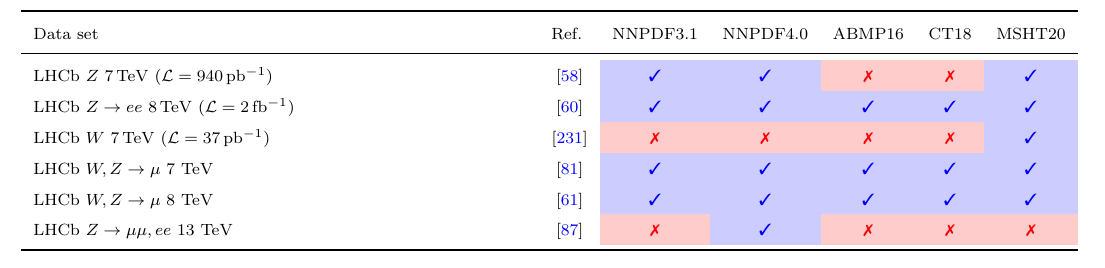
\includegraphics[width=0.9\textwidth]{lhcb_data_table}
    \end{columns}
\end{frame}





\begin{frame}{Performance benefit - time per replica}
  \begin{table}
     \renewcommand{\arraystretch}{1.50}
    \centering
    \begin{tabular}{c | c | c | c} \toprule
      & NNPDF3.1  & NNPDF4.0 (CPU) & NNPDF4.0  (GPU) \\
            \midrule
      Fit timing per replica    & 15.2 h        & 38 min        & 6.6 min \\ \hline
             Speed up factor    & 1        &  24      & 140 \\ \hline
      RAM use &  1.5 GB          &  6.1 GB                 & NA  \\ \bottomrule
    \end{tabular}
  \end{table}
  \vspace*{1em}
\end{frame}


\begin{frame}[t]{Hyperoptimization: the reward function}
    \begin{columns}[T]
        \begin{column}{0.48\textwidth}
            \vspace{\topsep}
            Choosing as the hyperoptimization target the $\chi^2$ of fitted data results in overfitting.
        \end{column}
        \begin{column}{0.48\textwidth}
            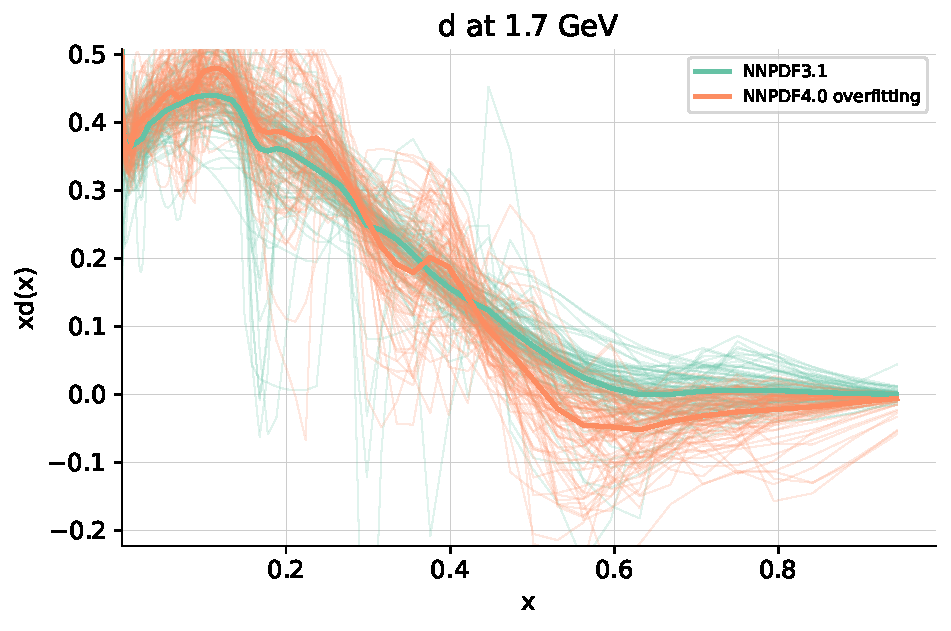
\includegraphics[width=0.9\textwidth]{overfit_nnpdf31}
        \end{column}
    \end{columns}
\end{frame}



\begin{frame}[t]{Hyperoptimization: the reward function}
    \begin{columns}[T]
        \begin{column}{0.48\textwidth}
            \vspace{\topsep}
            Choosing as the hyperoptimization target the $\chi^2$ of fitted data results in overfitting.\\
      \vspace*{2em}			
      We solve this using \textbf{k-fold cross-validation}:
      \begin{enumerate}
          \item Divide the data into $k$ {representative subsets}
          \item Fit $k-1$ sets and use $k$-th as test set
          \begin{itemize}
              \item[$\Rightarrow$] $k$ values of $\chi^2_\mathrm{test}$
          \end{itemize}
          \item Optimize the average $\chi^2_\mathrm{test}$ of the $k$ test sets
      \end{enumerate}
      \vspace*{0.5em}
      $\Rightarrow$ The hyperoptimization target is not based on data that entered the fit. 
        \end{column}
        \begin{column}{0.48\textwidth}
            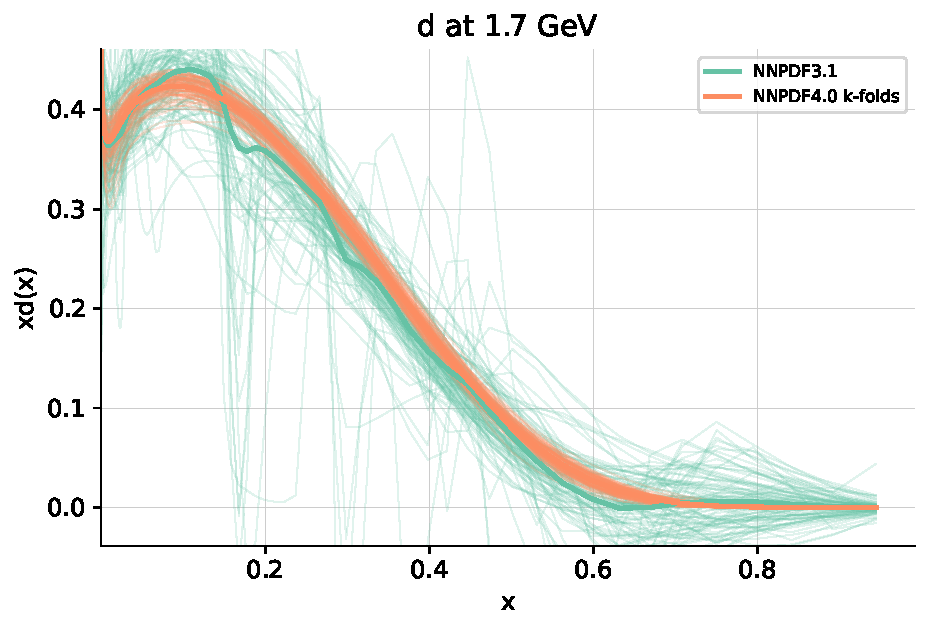
\includegraphics[width=0.9\textwidth]{best_model_vs_nnpdf31}
            \begin{itemize}
                \item No overfitting\\
          \vspace*{0.2em}
          \item Compared to NNPDF3.1:
          \begin{itemize}
              \item Increased stability
              \item Reduced uncertainties 
          \end{itemize}
      \end{itemize}
        \end{column}
    \end{columns}
\end{frame}



\begin{frame}{Parametrization basis independence}
    \begin{columns}
        \begin{column}[T]{0.48\textwidth}
        \vspace*{0pt}%
	        \begin{center}
	            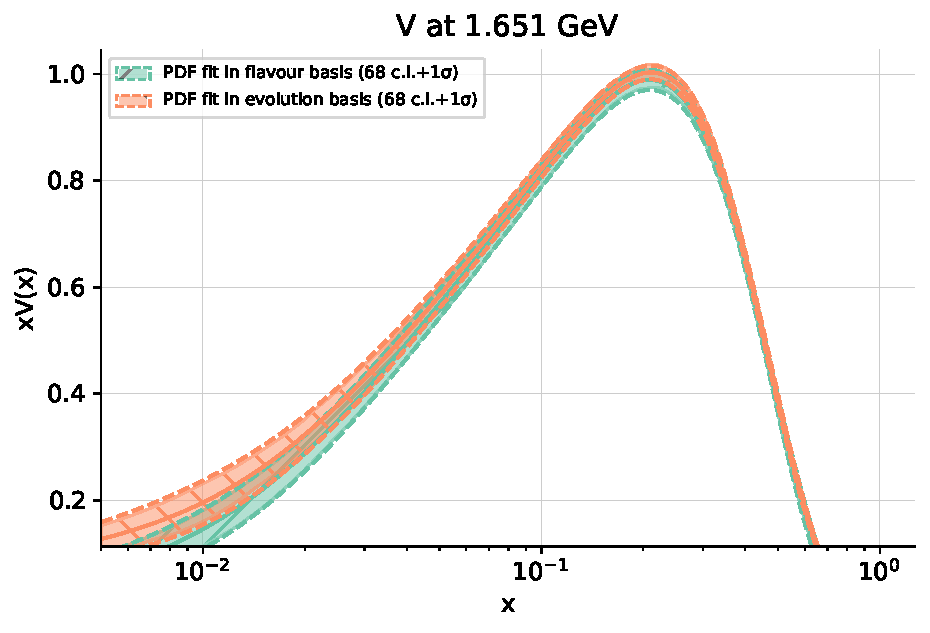
\includegraphics[width=0.8\textwidth]{flavour_evolution_V} \\
	        \end{center}
        \end{column}
        \begin{column}[t]{0.48\textwidth}
        \vspace{0pt}%
	        \begin{center}
	            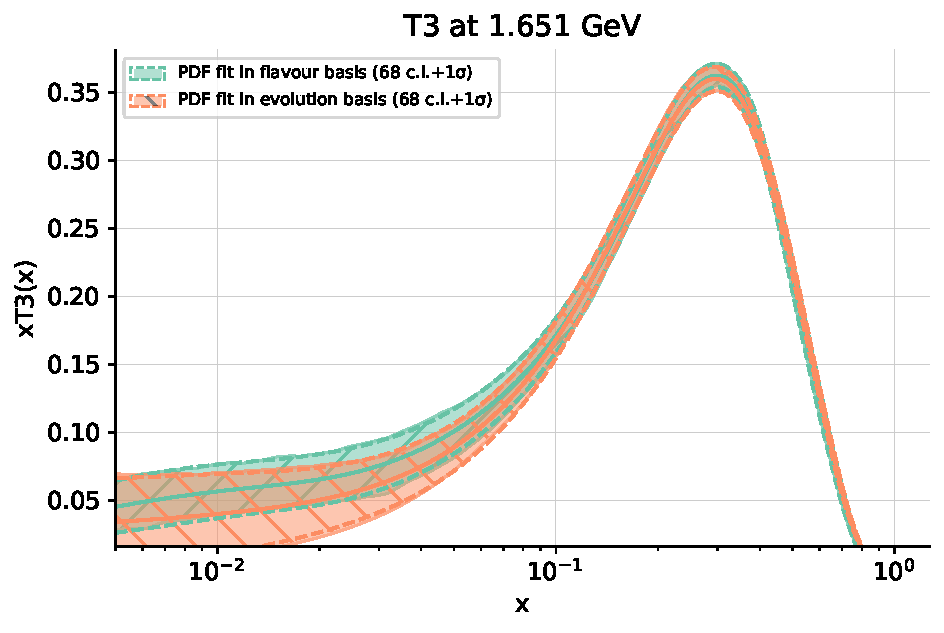
\includegraphics[width=0.8\textwidth]{flavour_evolution_T3} \\
	        \end{center}
        \end{column}
    \end{columns}
    \begin{columns}
        \column{0.4\linewidth}
		    Evolution Basis:
		    {\footnotesize
		    \begin{fleqn}
		    \begin{align*}
		       \qquad x V\left(x, Q_{0}\right) &\propto \mathrm{NN}_{V}(x)\\
		        x T_{3}\left(x, Q_{0}\right) &\propto \mathrm{NN}_{T_{3}}(x)
		    \end{align*}
		    \end{fleqn}
		    }
        \column{0.55\linewidth}
            \begin{block}{}
                Different strategies to parametrize the quark PDF flavour combinations leave the uncertainties essentially unchanged
            \end{block}
    \end{columns}
    \vspace*{-0.5em}
    Flavour Basis:
    {\footnotesize
    \begin{fleqn}
    \begin{align*}
        \qquad x V\left(x, Q_{0}\right) &\propto\left(\mathrm{NN}_{u}(x)-\mathrm{NN}_{\bar{u}}(x)+\mathrm{NN}_{d}(x)-\mathrm{NN}_{\bar{d}}(x)+\mathrm{NN}_{s}(x)-\mathrm{NN}_{\bar{s}}(x)\right) \\
        x T_{3}\left(x, Q_{0}\right) &\propto\left(\mathrm{NN}_{u}(x)+\mathrm{NN}_{\bar{u}}(x)-\mathrm{NN}_{d}(x)-\mathrm{NN}_{\bar{d}}(x)\right)
    \end{align*}
    \end{fleqn}
    }
\end{frame}


\begin{frame}[t]{Closure test}{See \href{https://arxiv.org/pdf/2103.08606.pdf}{\color{blue}Eur.Phys.J.C 82 (2022); arxiv:2111.05787}}
    Closure test of a known input assumption
    \begin{enumerate}
        \item Assume a ``true'' underlying PDF (e.g. a single PDF replica)
        \item Produce data distributed according to the experimental covariance matrices
        \item Perform a fit to this data
    \end{enumerate}
    \vspace*{1em}
    Examples of statistical estimators:

    \begin{itemize}
        \item \textbf{Bias}: squared difference between central value and true observable\\
        \textbf{Variance}: variance of the model predictions\\
        Faithful uncertainties require $E[\textrm{bias}]=\textrm{variance}$
        \item Is truth within one sigma in 68\% of cases?
    \end{itemize}
    \vspace*{1em}
    % Requires many fits - now possible with the new code
    \begin{textblock*}{\textwidth}(10cm,6cm) % {block width} (coords)
        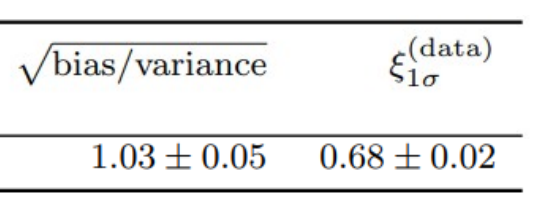
\includegraphics[width=5cm]{closure_results}
    \end{textblock*}
\end{frame}




\begin{frame}[t]{Impact of the new data}
	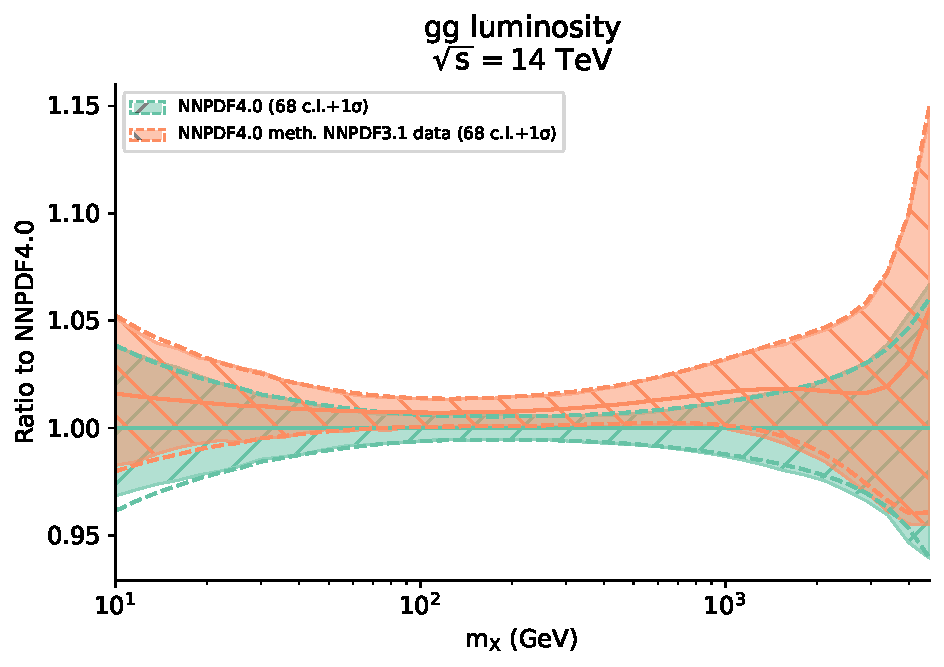
\includegraphics[width=0.45\textwidth]{lumi1d_gg_NNPDF40meth_NNPDF31data}
	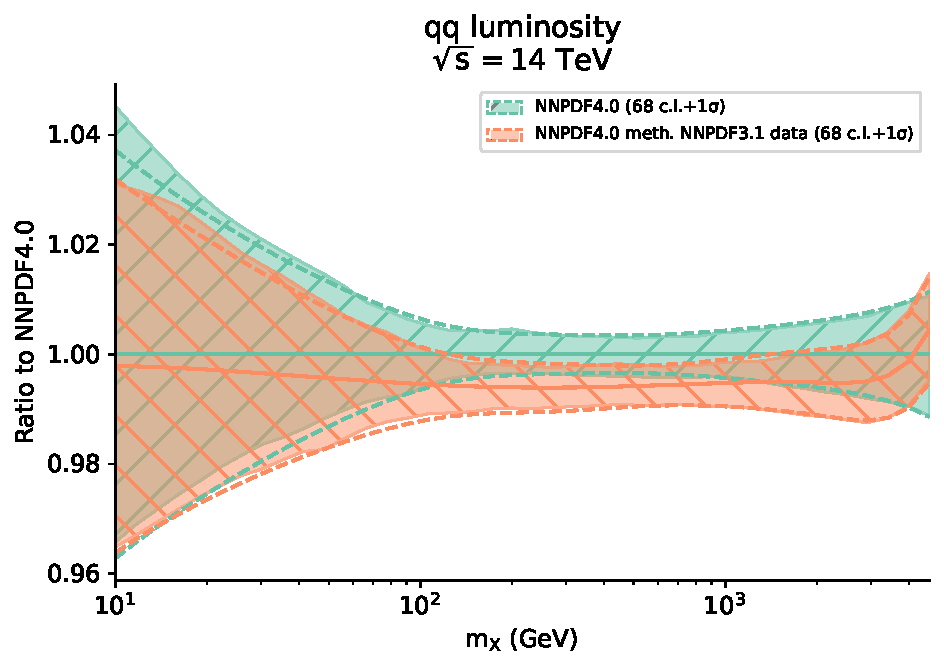
\includegraphics[width=0.45\textwidth]{lumi1d_qq_NNPDF40meth_NNPDF31data}
	Individual datasets have a limited impact, but collectively they result in:
	\begin{itemize}
	    \item Moderate reduction of PDF uncertainties
	    \item Shifts in central value at the one-sigma level
	\end{itemize}
\end{frame}


\begin{frame}[t]{Impact of the new fitting methodology}
	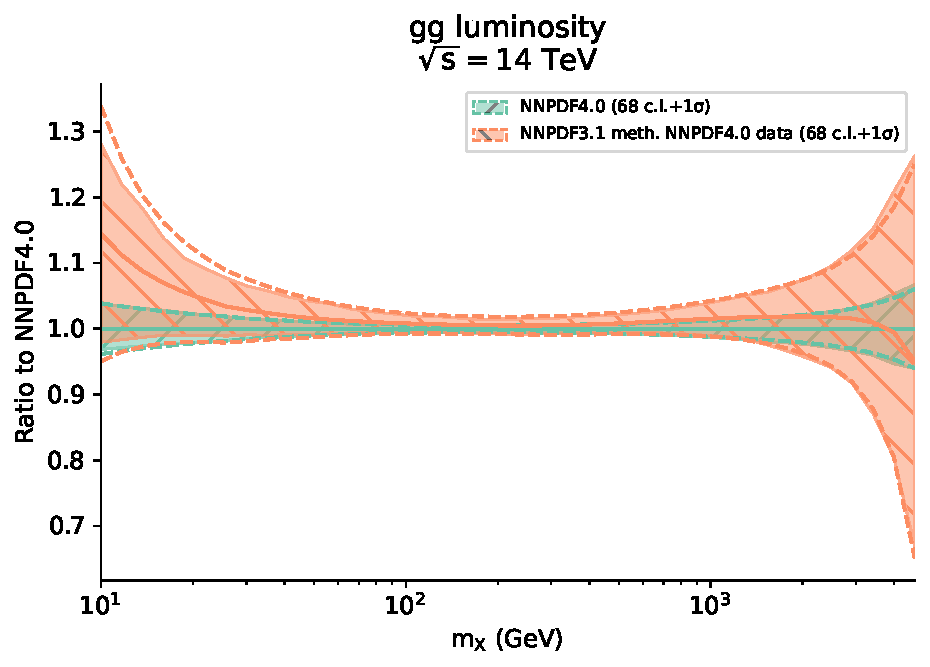
\includegraphics[width=0.45\textwidth]{lumi1d_gg_NNPDF31meth_NNPDF40data}
	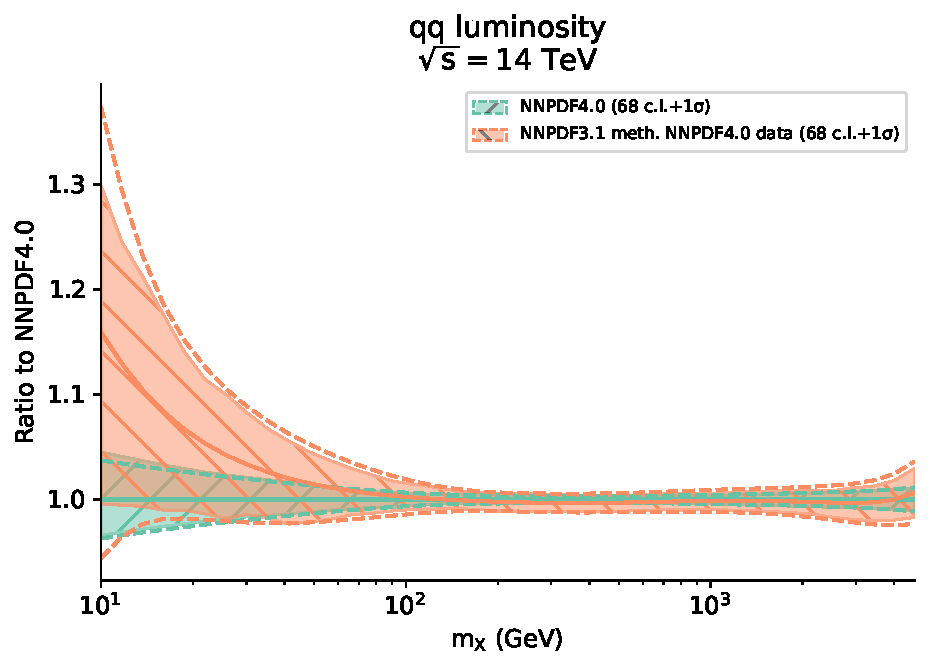
\includegraphics[width=0.45\textwidth]{lumi1d_qq_NNPDF31meth_NNPDF40data}
	\begin{columns}
	    \column{0.45\linewidth}
			\begin{itemize}
	    	        \item Significant reduction of PDF uncertainties
		        \item Good agreement between the central values
		    \end{itemize}
        \column{0.5\linewidth}
            \begin{block}{}
                \fontsize{7}{6}\selectfont
                PDF uncertainties are validated using closure tests and future tests\\
                Validation tests successful for both NNPDF4.0 and NNPDF3.1 
            \end{block}
    \end{columns}
\end{frame}



\begin{frame}{The (negligible) impact of datasets with tension}
    Excluding datasets with large $({\chi^{2}-1})/{\sigma_{\chi^{2}}}$ one at a time and combining the resulting PDFs following the conservative PDF4LHC15 prescription shows stability at the level of statistical fluctuations.
    \begin{columns}
        \begin{column}[T]{0.32\textwidth}
            \centering
            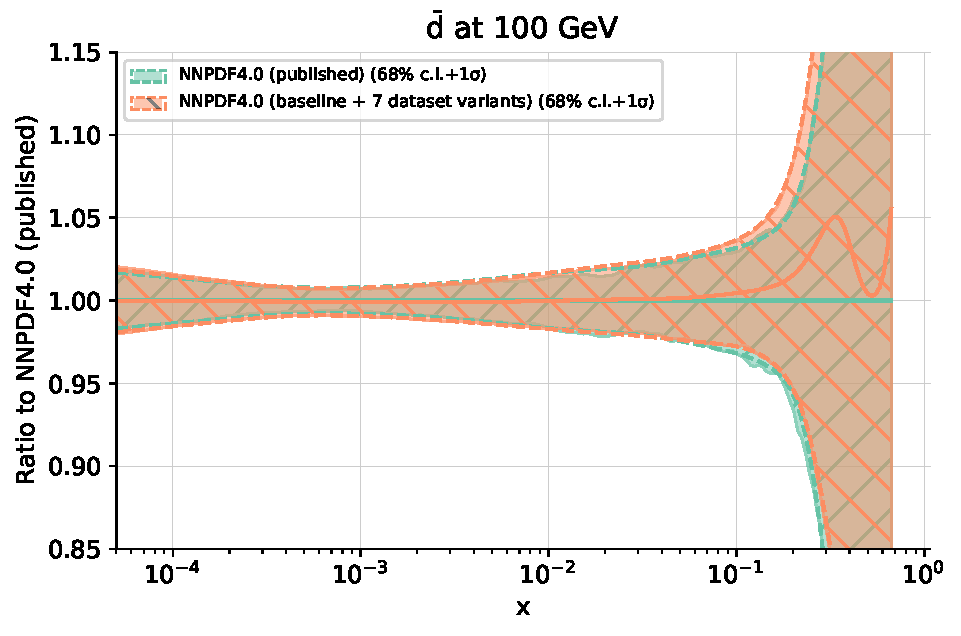
\includegraphics[width=0.9\textwidth]{env_bard.pdf}\\
            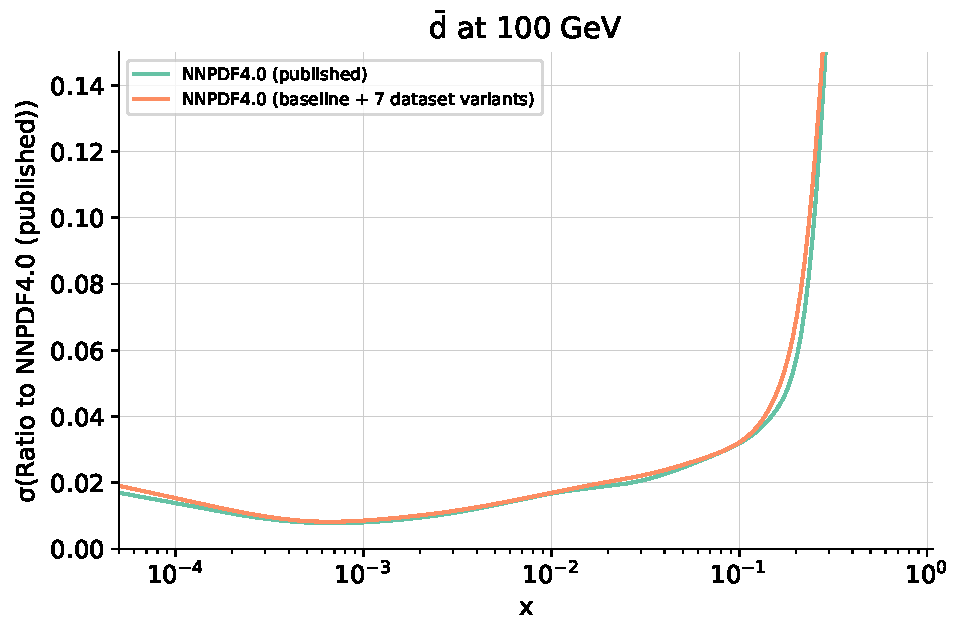
\includegraphics[width=0.9\textwidth]{envu_bard.pdf}
        \end{column}
        \begin{column}[T]{0.32\textwidth}
            \centering
            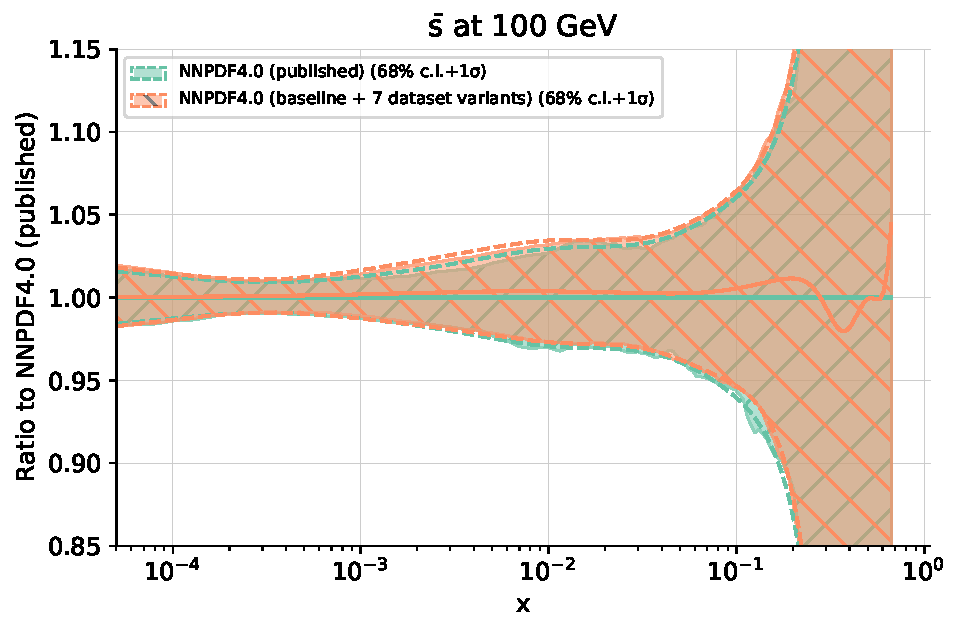
\includegraphics[width=0.9\textwidth]{env_bars.pdf}\\
            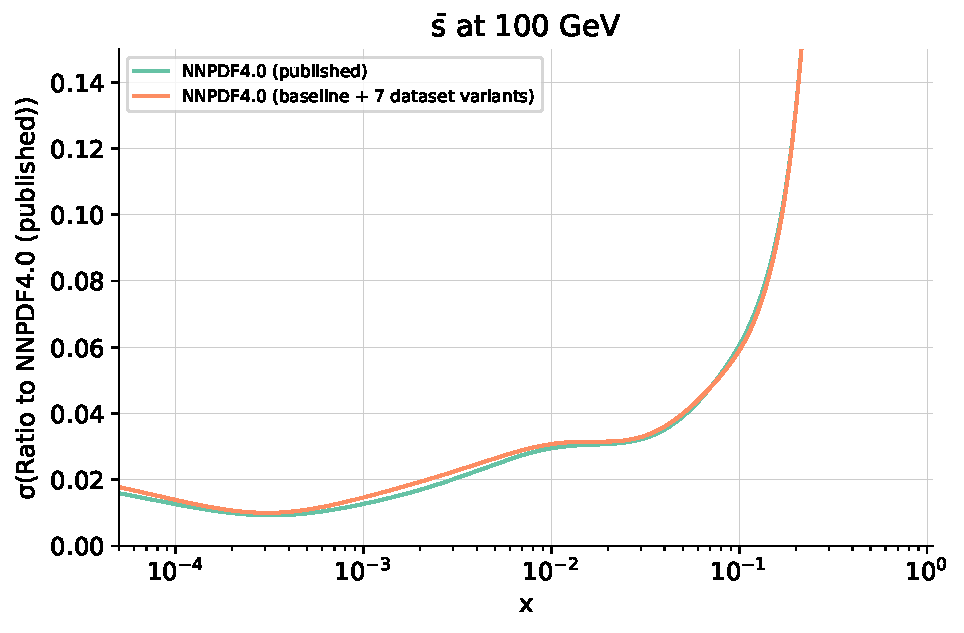
\includegraphics[width=0.9\textwidth]{envu_bars.pdf}
        \end{column}
        \begin{column}[T]{0.32\textwidth}
            \centering
            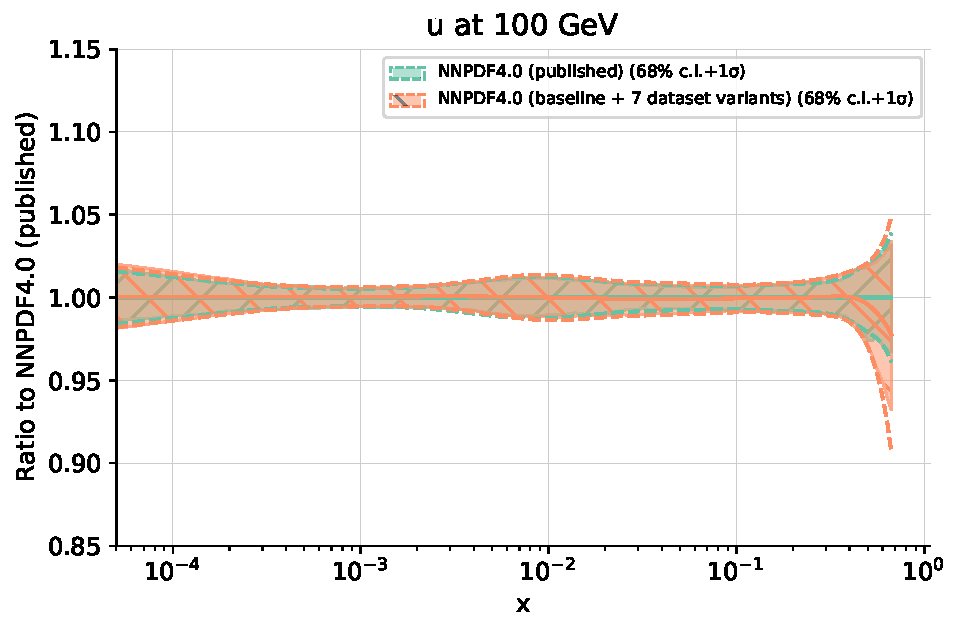
\includegraphics[width=0.9\textwidth]{env_u.pdf}\\
            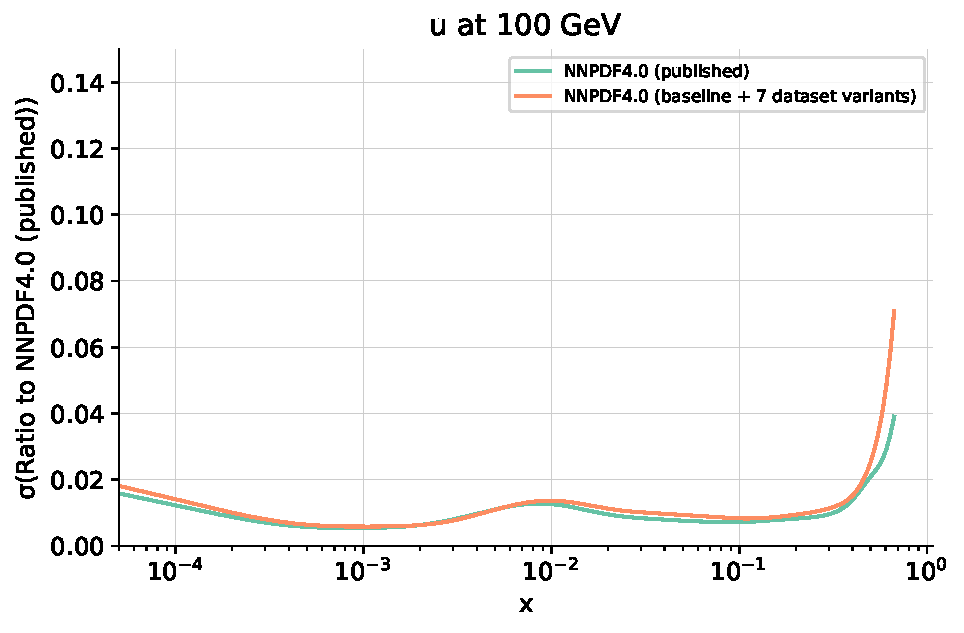
\includegraphics[width=0.9\textwidth]{envu_u.pdf}
        \end{column}
    \end{columns}
\end{frame}


\begin{frame}{Envelope of fits with different parametrization bases}
    Different strategies to parametrize the PDF flavour combinations lead to the same result
    \vspace*{-1em}
    \begin{columns}
        \begin{column}[T]{0.32\textwidth}
          \begin{center}
              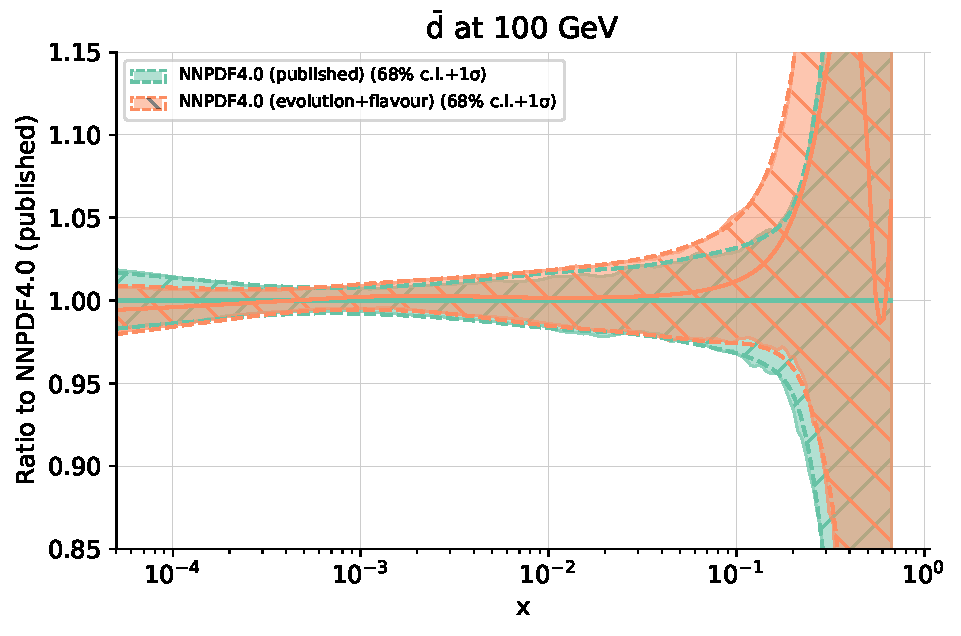
\includegraphics[width=0.95\textwidth]{efenv_bard.pdf} \\
              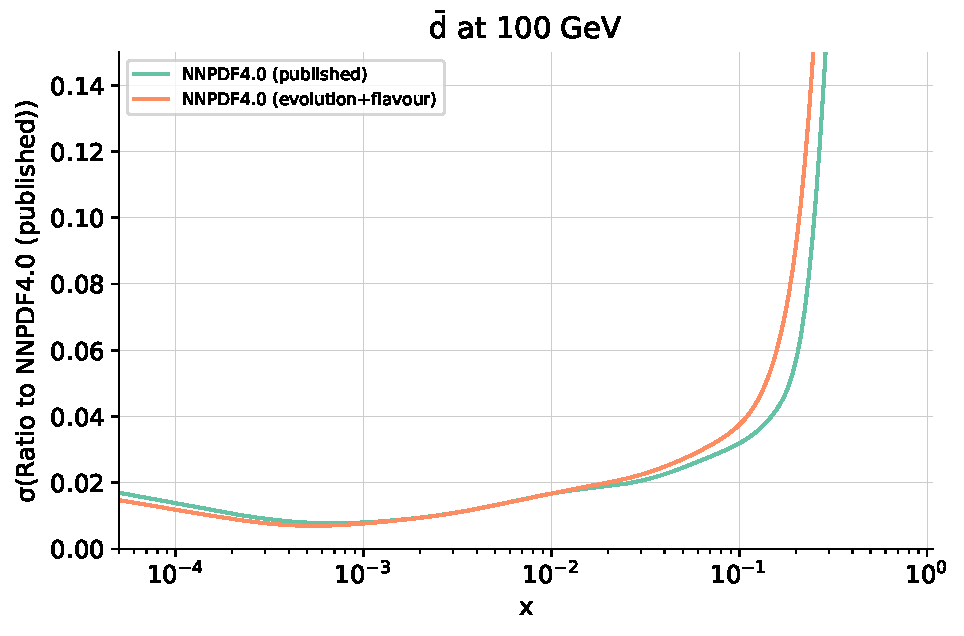
\includegraphics[width=0.95\textwidth]{efenvu_bard.pdf} 
          \end{center}
        \end{column}
        \begin{column}[t]{0.32\textwidth}
          \begin{center}
              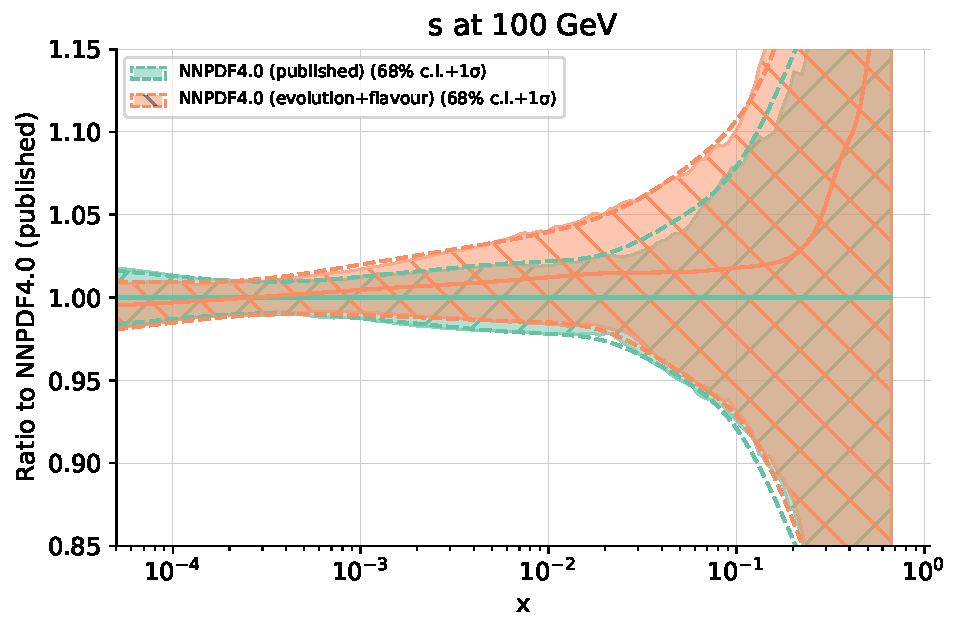
\includegraphics[width=0.95\textwidth]{efenv_s.pdf} \\
              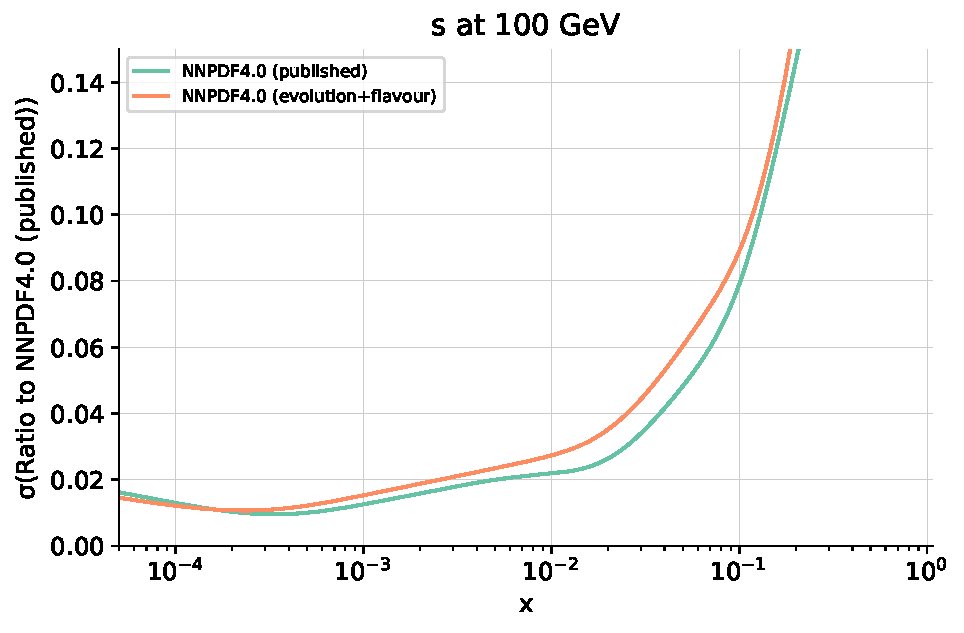
\includegraphics[width=0.95\textwidth]{efenvu_s.pdf} 
          \end{center}
        \end{column}
        \begin{column}[t]{0.32\textwidth}
            \begin{center}
                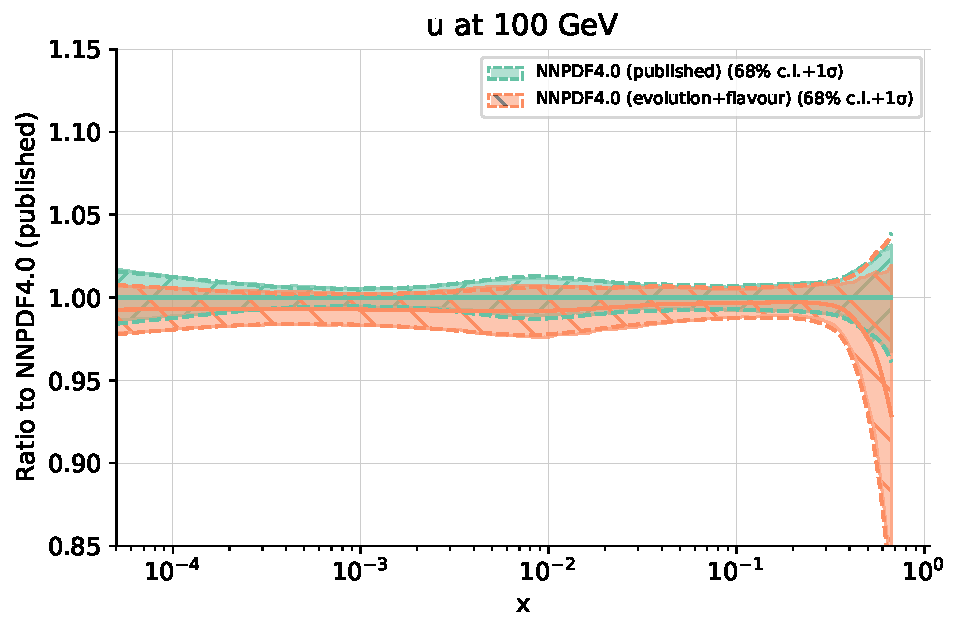
\includegraphics[width=0.95\textwidth]{efenv_u.pdf} \\
                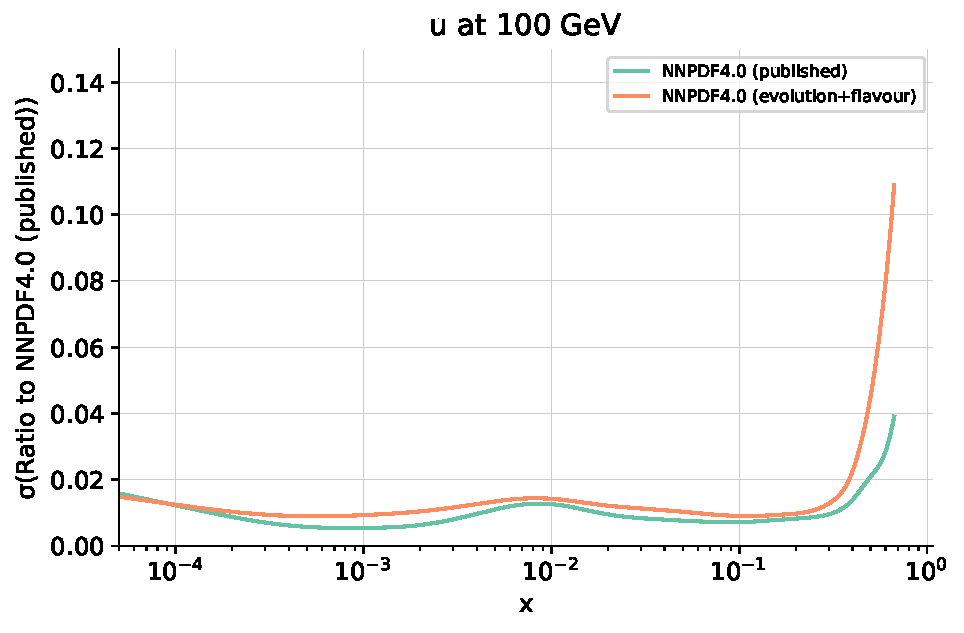
\includegraphics[width=0.95\textwidth]{efenvu_u.pdf} 
            \end{center}
          \end{column}
    \end{columns}
\end{frame}


\begin{frame}{Understanding the $\chi^2$ distribution}
    \begin{columns}
        \begin{column}[T]{0.48\textwidth}
            \centering
            Experimental $\chi^2$
            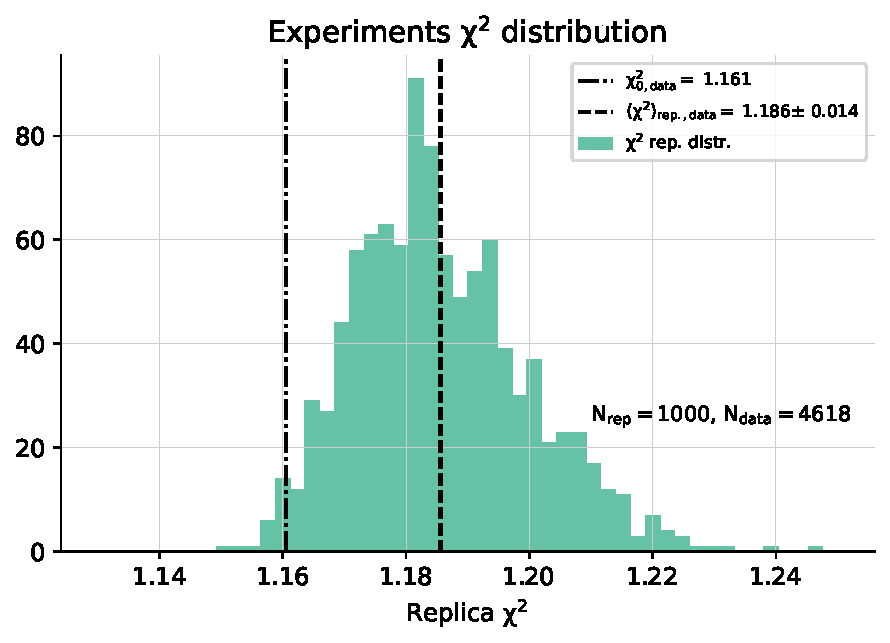
\includegraphics[width=\textwidth]{c2hist.pdf}
        \end{column}
        \begin{column}[T]{0.48\textwidth}
            \centering
            $t_0$ $\chi^2$
            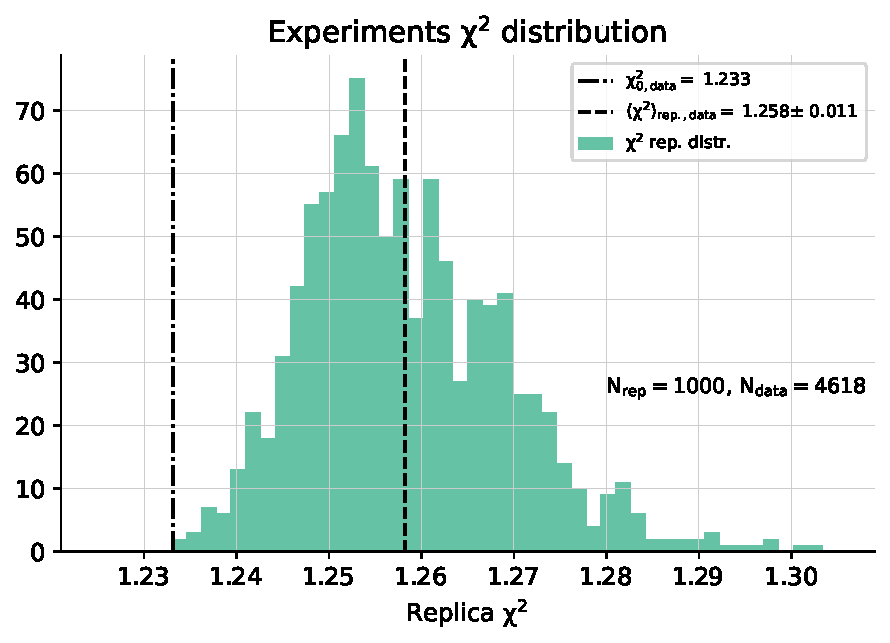
\includegraphics[width=\textwidth]{c2histt0.pdf}
        \end{column}
    \end{columns}
\end{frame}


\begin{frame}[t]{Impact of positivity on the PDFs}
    \begin{center}
        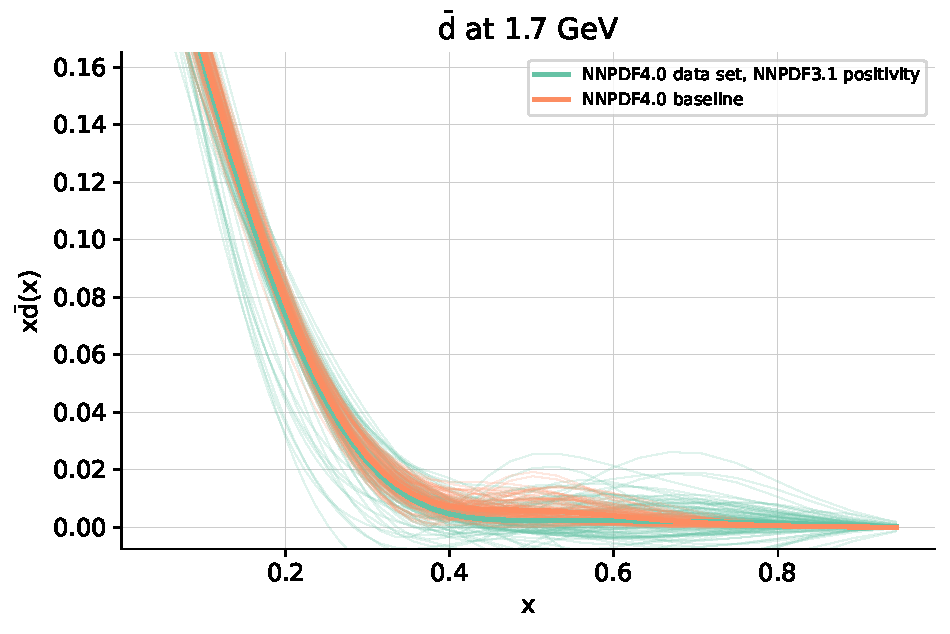
\includegraphics[width=0.6\textwidth]{dbpos.pdf}
    \end{center}
\end{frame}



\begin{frame}{More implications for phenomenology}
    \begin{columns}
        \begin{column}[T]{0.32\textwidth}
            \centering
            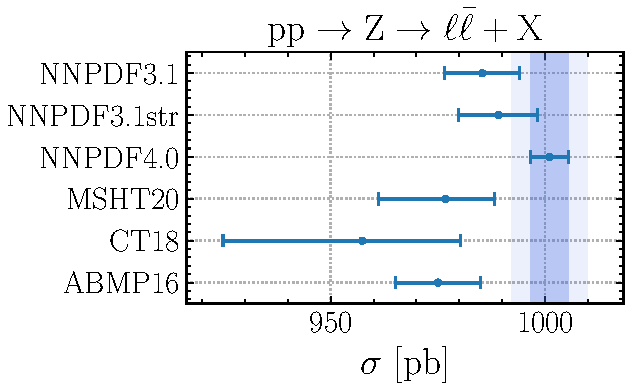
\includegraphics[width=\textwidth]{NNPDF_DY_14TEV_40_PHENO-integrated.pdf}
        \end{column}
        \begin{column}[T]{0.32\textwidth}
            \centering
            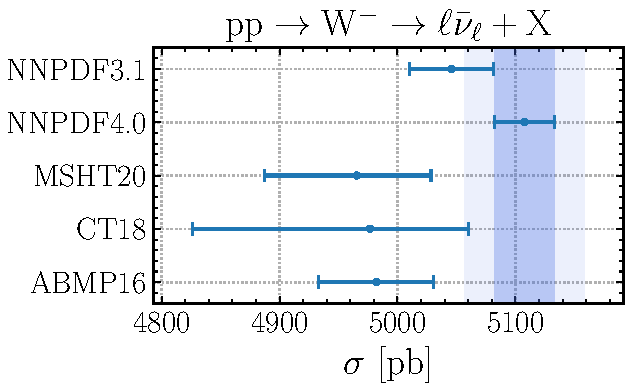
\includegraphics[width=\textwidth]{NNPDF_WM_14TEV_40_PHENO-integrated.pdf}\\
        \end{column}
        \begin{column}[T]{0.32\textwidth}
            \centering
            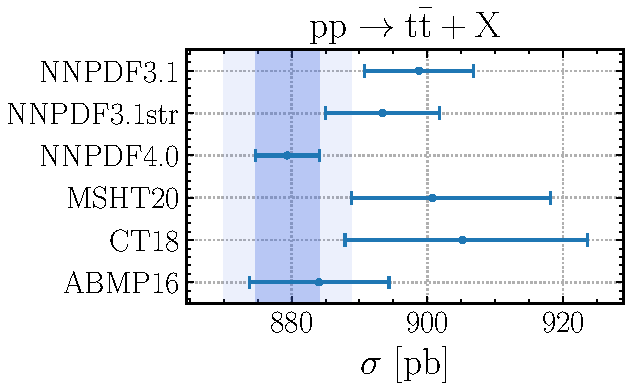
\includegraphics[width=\textwidth]{NNPDF_TTB_14TEV_40_PHENO-integrated.pdf}
        \end{column}
    \end{columns}
\end{frame}


\begin{frame}{Small $M_{ll}$}
    \centering
    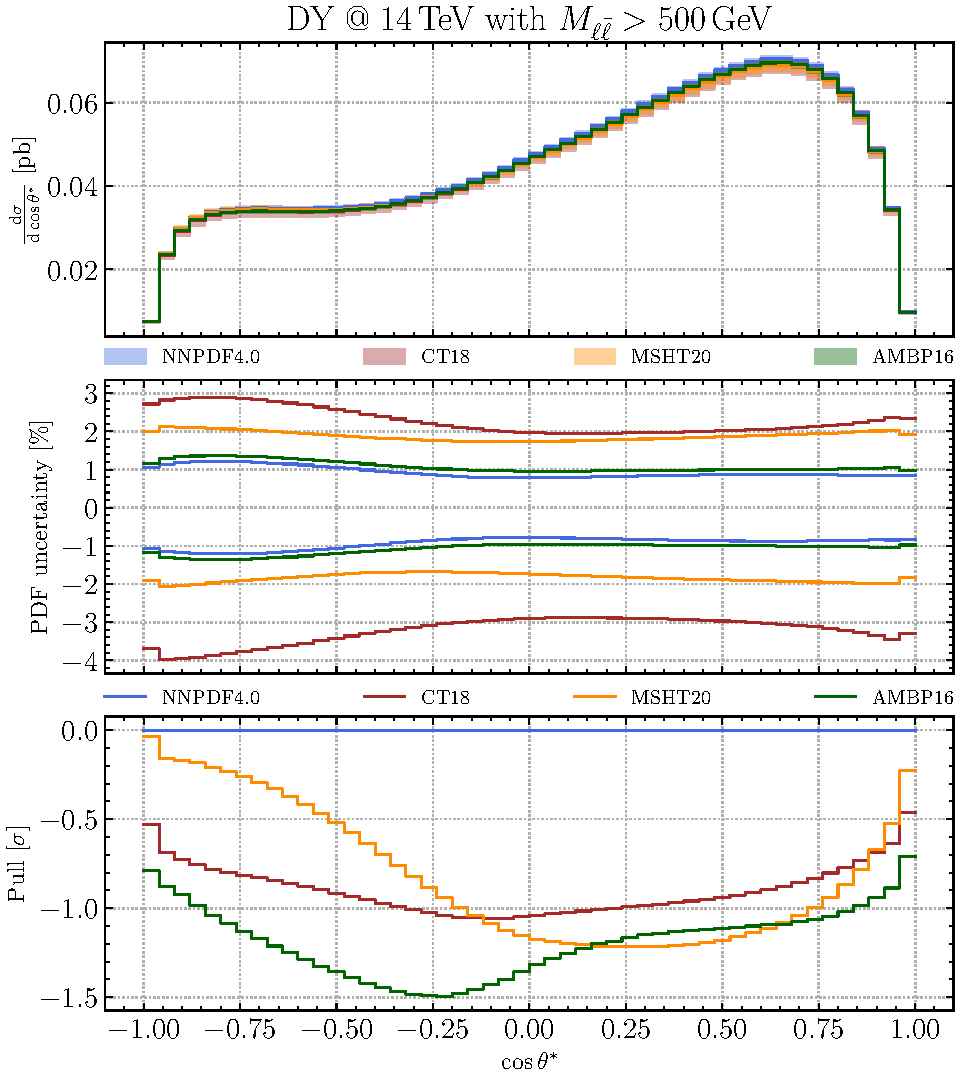
\includegraphics[width=0.32\textwidth]{CMS_DY_14TEV_MLL_0500_COSTH}
    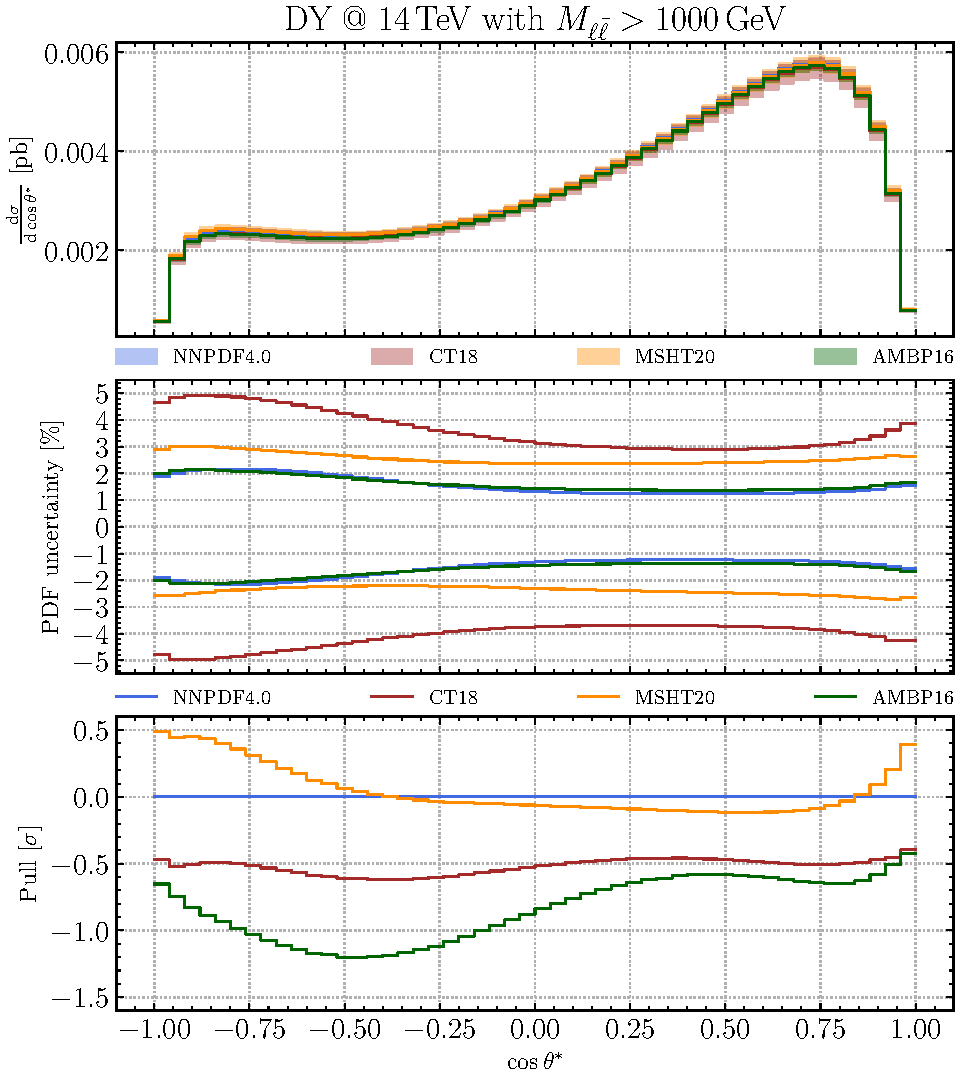
\includegraphics[width=0.32\textwidth]{CMS_DY_14TEV_MLL_1000_COSTH}
    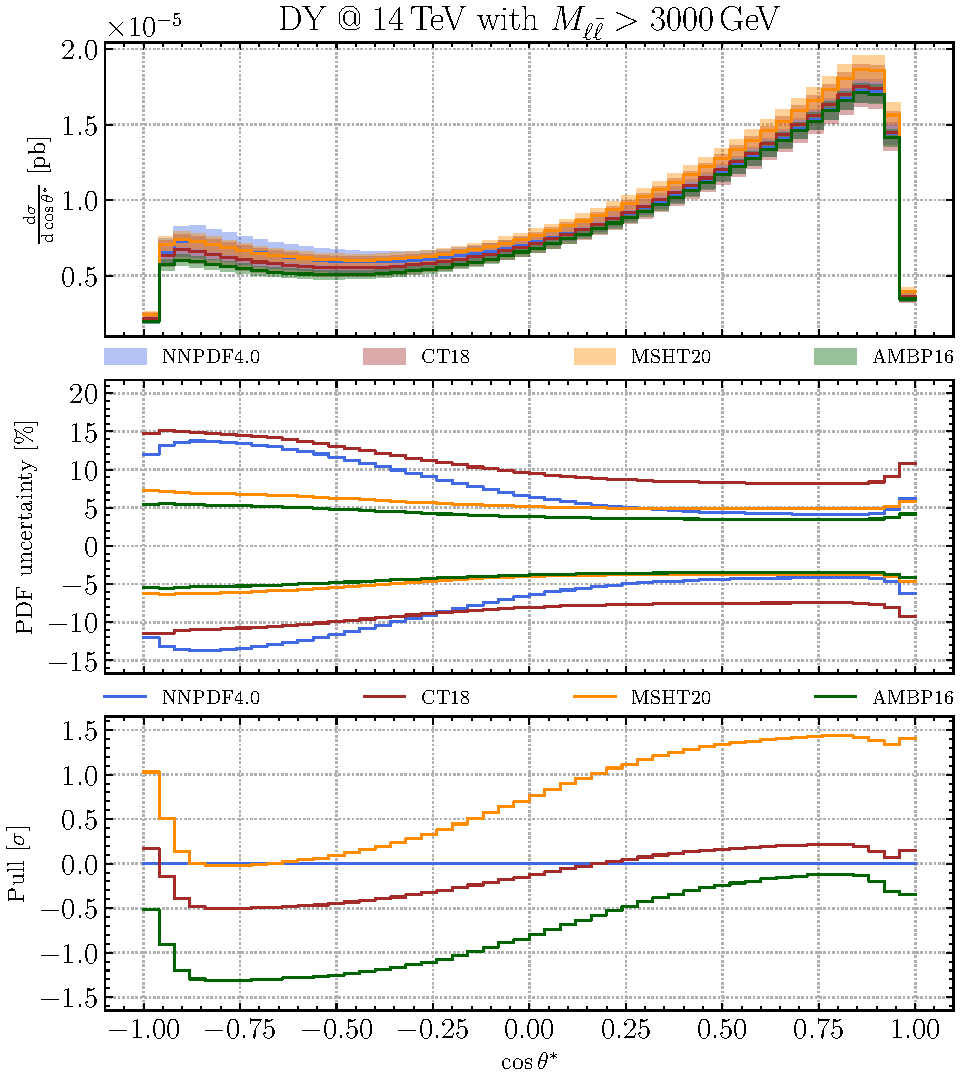
\includegraphics[width=0.32\textwidth]{CMS_DY_14TEV_MLL_3000_COSTH}\\
    Small uncertainties in the data region
\end{frame}


